% !TEX root = ../main.tex

\chapter{Introduction}
\label{ch:introduction}

\section{Black-Box Optimization}
\subsection{Evolution Strategies}
Evolution Strategies (ES) ...

\subsection{Covariance Matrix Adaptation Evolution Strategy}
Covariance Matrix Adaptation Evolution Strategy (CMA-ES) ...

\section{Function Approximators}
We can represent many problems in machine learning as a function mapping an input space into an output space. This underlying function is the output of the learning process of an algorithm and is often called the \textit{target function}. Optimally, we would derive the formula of the function explicitly. However, even though we suspect that such a function exists, we usually do not have enough information to derive a formula. Thus, we aim to approximate the target function with function approximators by using the available data. In general, we can apply any function approximator. However, each function approximator has its advantages and limitations. For example, some may be prone to local optimum. Depending on the task, this could prevent us from finding a good approximation.

\subsection{Neural Networks}
Neural networks are machine learning algorithms inspired by the functionalities of the brain. They consist of connected neurons or nodes that imitate the biological neurons of the brain sending signals to each other. In a neural network, the neurons are arranged in connected layers. A network has at least an input and an output layer. We can further expand it with one or more hidden layers. Depending on the model, the connectivity between the layers differs. Figure~\ref{fig:neural_network_sketch} shows a sketch of a network with three hidden layers that are fully connected.
\begin{figure}[ht]
\centering
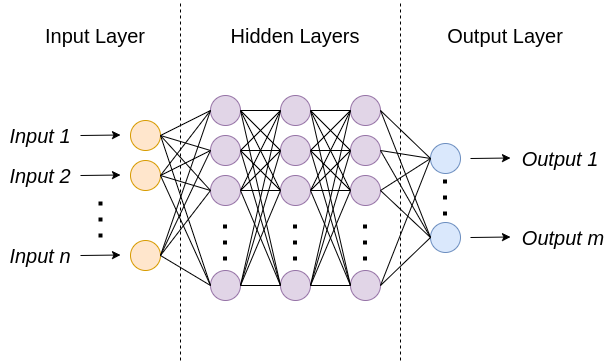
\includegraphics[width=.7\textwidth]{neural_network_sketch}
\caption[Sketch of a Neural Network]{
  \textbf{Sketch of a neural network.}
  The image shows a sketch of a neural network with three fully connected hidden layers.
}
\label{fig:neural_network_sketch}
\end{figure}
Each neuron holds an associated weight and threshold. It receives an input and outputs the sum of weighted inputs. If this sum is greater than the associated threshold, the neuron gets activated.

A neural network with one or more hidden layers defines a non-linear function. It is theoretically able to represent any function. Thus, it is a \textit{generic function approximator}.
Neural networks are highly expressive and flexible. They are applied successfully in many areas. A large part of the success of neural networks can be traced to the use of \textit{backpropagation}. Backpropagation uses information from the previous epoch (i.e. iteration) to adjust the weights of the network using the error gradient. However, neural networks also come with a few limitations or disadvantages. The backpropagation algorithm requires the calculation of an accurate gradient. Depending on the problem, this can be a challenging task. Furthermore, there is a lack of understanding. The output of a neural network is often incomprehensible because of its complex structure.

\todo[inline]{Explain more, e.g. bias, generic function approximator \\ Improve NN Figure}



\subsection{Polynomial}
In mathematics, a polynomial is the sum of powers in one or more variables multiplied by coefficients. It can be used to express linear combinations. In the following, we will mainly work with polynomials consisting of vectors instead of scalars. Thus, a polynomial $p(x)$ with $x$ being a vector of degree $n$ can be represented by
\[
  p(x) = \Sigma_{i=0}^{n} w_i^T (x_k^i)_{k \in I} \in \mathbb{R}, \ \ \ \ \ \ \ \ \ \ w_i, x \in \mathbb{R}^n, \ \ I = \{0, ..., n\},
\]
where $w_i$ are constant coefficients. Polynomials are relatively simple mathematical expressions and offer some significant advantages: their derivative and indefinite integral are easy to determine and are also polynomial. Due to their simple structure, polynomials can be valuable to analyze more complex functions using polynomial approximations. \textit{Taylor's theorem} tells us that we can locally approximate any $k$-times differentiable function by a polynomial of degree $k$. We call this approximation \textit{Taylor polynomial}. Furthermore, the \textit{Weierstrass approximation theorem} says that we can uniformly approximate every continuous function defined on a closed interval by a polynomial. Other applications of polynomials are \textit{polynomial interpolation} and \textit{polynomial splines}. Polynomial interpolation describes the problem of constructing a polynomial that passes through all given data points. Polynomial splines are piecewise polynomial functions that can also be used for spline interpolation.

\todo[inline]{Include theorems}

\subsection{Fourier}

\subsection{Bézier}


\section{Previous Work}

\subsection{Benchmarks in Reinforcement Learning}
\label{ssec:benchmarks}
When developing a novel algorithm, it is important to compare our results with existing models. For this evaluation, we need standard benchmark problems. These are a set of standard optimization problems. OpenAI Gym \footnote{\url{gym.openai.com}} is a toolkit created for exactly this scenario. It contains a collection of benchmark problems with various levels of difficulty. However, not all benchmark problems are meaningful for the evaluation of an algorithm. If a problem is too trivial to solve, the results do not reflect the quality of the model adequately. We do not need to put a large amount of effort into the creation of a complex model for an easy-to-solve task.

In the paper \emph{Analyzing Reinforcement Learning Benchmarks with Random Weight Guessing} (\citet{oller_analyzing_2020}), the authors analyze and visualize the complexity of standard RL benchmarks based on score distribution. They tested their approach on the five Classic Control benchmark problems from the OpenAI Gym interface: \verb|CartPole|, \verb|Acrobot|, \verb|Pendulum|, \verb|MountainCar|, and \verb|MountainCarCon-| \verb|tinuous|. Given an RL environment, the authors conducted a fixed series of experiments. For these experiments, they used three neural network architectures ($N_{architectures}=3$): a network without any hidden layers (0 HL), a network with a single hidden layer of 4 units (1 HL, 4 HU), and a network with two hidden layers of 4 units each (2 HL, 4 HU). With these, they cover a variety of network models that are suited to solve the given tasks. The evaluation should be as objective as possible and should not include bias in the data. To achieve this, the authors did not include any learning opportunities for the network models. Instead, they chose the network weights i.i.d. from the standard normal distribution $\mathcal{N}(0,1)$ with Random Weight Guessing (RWG). This approach assures randomness and no directed learning. The goal of the paper was not to further analyze the network models but to investigate the benchmark problems themselves. With this in mind, they initialized $10^4$ samples ($N_{samples}=10^4$) with different random weights. The number of samples would be too large for a reasonable learning strategy. However, the large number of samples serves a different purpose than optimizing the results. Instead, the aim is to draw statistical conclusions. Each of these samples of a neural network represents a controller that maps observations to actions in the environment. Later in this thesis, I will explore function approximators other than neural networks representing the controller. In the paper, the authors tested the controllers for each environment during 20 independent episodes ($N_{episodes}=20$). For each episode, they saved the score in the score tensor $S$. Algorithm~\ref{alg:environment-evaluation} illustrates the procedure with pseudocode.

\begin{algorithm}
\caption{Evaluation process taken from \citet{oller_analyzing_2020}}
\begin{algorithmic}[1]
\State Initialize environment
\State Create array $S$ of size $N_{architectures} \times N_{samples} \times N_{episodes}$
\For{$n = 1,2,...,N_{samples}$}
    \State Sample NN weights randomly from $\mathcal{N}(0,1)$
    \For{$e=1,2,...,N_{episodes}$}
      \State Reset the environment
      \State Run episode with NN
      \State Store accured episode reward in $S_{a,n,e}$
    \EndFor
\EndFor
\end{algorithmic}
\label{alg:environment-evaluation}
\end{algorithm}

After the authors obtained the scores, they calculated the mean performance over all episodes from a sample and its variance. These statistics are significant insights. They can reveal how stable the network models are in completing a given task. A low mean value suggests that, in general, the network cannot complete the task. The variance gives us further insight into the score distribution. It illustrates how spread out the scores are from their respective mean score. A high value means that we have high variability. A controller is valuable if it can solve a specific task reliably and stable. Therefore, we strive for a high value for the mean and a low value for the variance. However, training a network with random weight guessing should generally not result in a stable controller. If this is the case, we can assume that the task to solve was too trivial and is not valuable for evaluation measurements. In the illustrations of the paper, the authors ranked the samples according to their mean scores. They then visualized their results with three plots: a log-scale histogram of the mean scores, a scatter plot of the sample scores over their rank, a scatter plot of score variance over the mean score.

I reproduced the results of the authors following the mentioned methodology. My findings for the environment \verb|CartPole| are displayed in Figure~\ref{fig:plots_reproduced}.
\begin{figure}[ht]
\centering
\begin{subfigure}{\textwidth}
  \centering
  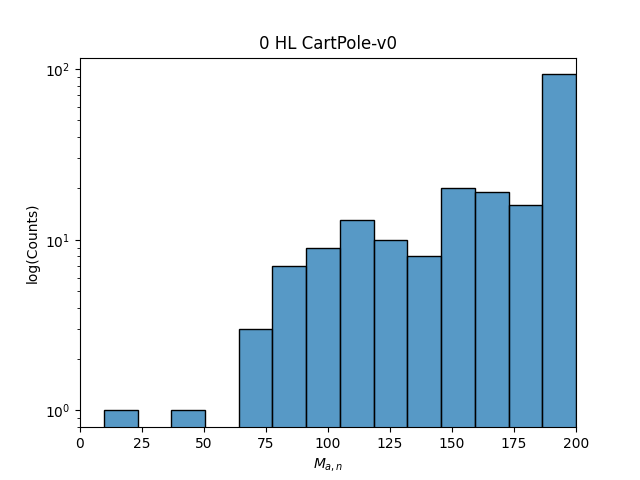
\includegraphics[width=0.329\textwidth]{reproduced_plots/histogram_zero_HL}
  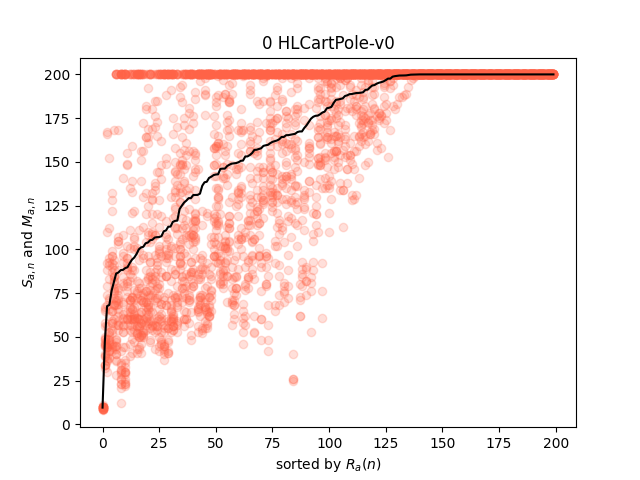
\includegraphics[width=0.329\textwidth]{reproduced_plots/scatter_score_zero_HL}
  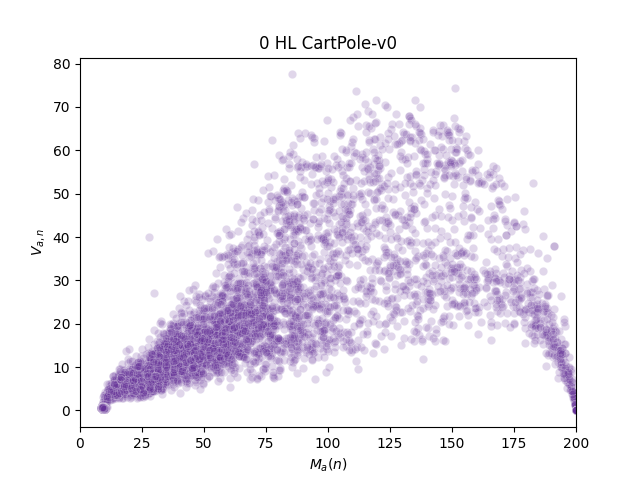
\includegraphics[width=0.329\textwidth]{reproduced_plots/scatter_variance_zero_HL}
    \caption{Results of network architecture without hidden layers}
    \label{fig:plots_reproduced_first}
\end{subfigure}
\begin{subfigure}{\textwidth}
  \centering
  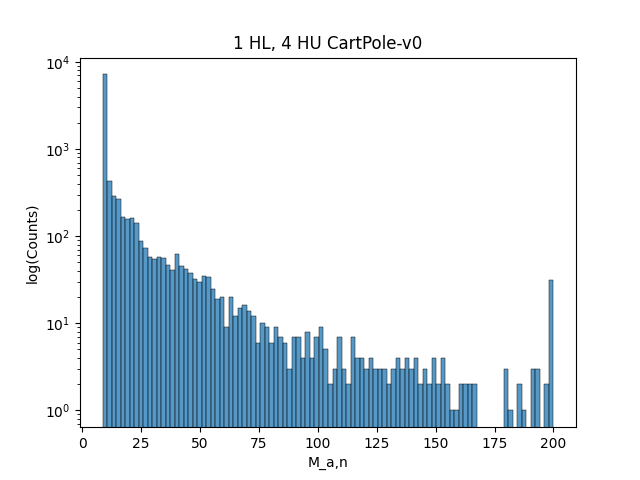
\includegraphics[width=0.329\textwidth]{reproduced_plots/histogram_one_HL}
  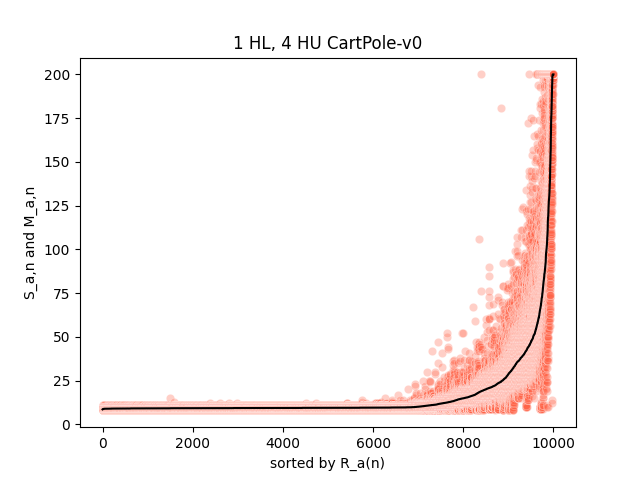
\includegraphics[width=0.329\textwidth]{reproduced_plots/scatter_score_one_HL}
  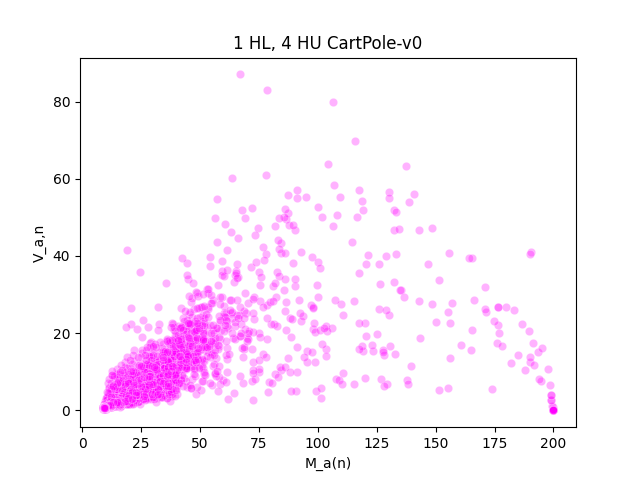
\includegraphics[width=0.329\textwidth]{reproduced_plots/scatter_variance_one_HL}
    \caption{Results of network architecture with one hidden layer}
    \label{fig:plots_reproduced_second}
\end{subfigure}
\begin{subfigure}{\textwidth}
  \centering
  \includegraphics[width=0.329\textwidth]{reproduced_plots/histogram_two_HL}
  \includegraphics[width=0.329\textwidth]{reproduced_plots/scatter_score_two_HL}
  \includegraphics[width=0.329\textwidth]{reproduced_plots/scatter_variance_two_HL}
    \caption{Results of network architecture with two hidden layers}
    \label{fig:plots_reproduced_third}
\end{subfigure}
\caption[Reproduced Plots]{
  \textbf{Results of the benchmark evaluation.}
   Results of the three network architectures illustrated as: (left images) a log-scale histogram of the mean scores, (middle images) a scatter plot of the sample scores over their rank, (right image) a scatter plot of score variance over the mean score
}
\label{fig:plots_reproduced}
\end{figure}
The figures illustrate the results for each of the three network architectures. Each row shows the histogram of the mean score values in the left image, the scatter plot of all scores over their rank in the image in the middle, and the scatter plot of the score variance over the mean score in the right image for a specific network architecture. There are few differences, but overall all network architectures deliver similar insights. The histogram plots show that the majority of networks receive a low score. Since the weights of the networks were chosen with RWG, this is rather unsurprising. But there is still a significant amount of networks that were able to achieve a high mean value or even the maximum value of 200. With a score of 200, the network was able to solve the task each episode. Therefore, the network could reliably solve the task without any learning technique involved. This should not be the case for a complex task. Furthermore, in the scatter plot in the middle, we can see that the line plot of the mean scores is a continuous increasing line without any jumps. Thus, a suited RL algorithm should generally be able to learn the task incrementally without converging into a local optimum. At the top of the scatter plot, we can see quite a few data points with a score of 200 that have a relatively low mean score. This indicates that a network that generally performs poorly can still solve the task with the right initialization conditions. Lastly, in the scatter plot on the right, we can see the distribution of the variance according to the mean value. On the left side, we have low scores of variance corresponding with a low mean value. These networks were consistently unable to achieve a high score. Without any training involved, we can expect most networks to be in this area. However, in the middle of the plot, the data points are spread out. For a high variance, the scores of a network differ highly from the mean value. Thus, we might get lucky and receive a high score depending on initialization conditions, but we might as well get a low score. These networks are inconsistent and unstable. On the right side of the scatter plot, we can see that the data points with a high mean value are mostly of low variance. Thus, to achieve a high mean value, the network needs consistency.

Interestingly, the usage of the bias had a relatively large impact on the performance of the network for the environment \verb|CartPole|. Without bias, the networks seem to achieve overall better scores. The plots in Figure~\ref{fig:plots_reproduced} illustrate the results without bias. For comparison, Figure~\ref{fig:comparison_bias} shows the results of a network with two hidden layers with the same configurations as before but this time including bias. In the paper, the authors conducted experiments with and without bias connection for all environments. They discovered that the amount of top performers increases when dropping bias for all five environments.
\begin{figure}[ht]
\centering
\includegraphics[width=0.329\textwidth]{with_bias_nn/histogram_two_HL}
\includegraphics[width=0.329\textwidth]{with_bias_nn/scatter_score_two_HL}
\includegraphics[width=0.329\textwidth]{with_bias_nn/scatter_variance_two_HL}
\caption[Impact of Bias]{
  \textbf{Impact of bias.}
  The figures show the performance of a network with two hidden layers with the same settings as before but here we include bias.
}
\label{fig:comparison_bias}
\end{figure}


\todo[inline]{Add plots from Acrobot \\ Adjust axis name in bias images, Change title of plots: , instead of with \\ Make text easier to read with padding \\ Make captions of figures more meaningful (why is this added? why shown like this?), refer to subplots}
